\ProvidesPackage{commands}
\documentclass[11pt]{article}
\usepackage{epstopdf}
\usepackage{subfigure,graphicx}
\usepackage{amsmath}
\usepackage{epsf}
\usepackage{amsfonts}
\usepackage{amssymb}
\usepackage{color}
\usepackage{mathtools}
\usepackage{placeins}
\usepackage{booktabs}
\usepackage{enumitem}
\usepackage{caption}
\usepackage[margin=0.8in, paperwidth=8.5in, paperheight=11in]{geometry}
\usepackage{amsfonts}
\usepackage{amsmath}
\usepackage{amsbsy}
\usepackage{authblk}
\usepackage{graphicx}
\usepackage{listings}
\usepackage{array}
\usepackage{titlesec}
\usepackage{amssymb}
\usepackage{bm}
\usepackage{mathtools}
\usepackage{titlesec}

\usepackage[latin1]{inputenc}\newcommand{\bs}[1]{\boldsymbol{#1}}
\newcommand{\del}[2]{\frac{\partial {#1}}{\partial {#2}}}
\newcommand{\D}[2]{\frac{D^{\overline{\alpha}}}{\overline{\alpha !}}{#1}(#2,#2)\ {\bf x}^{\overline{\alpha}}}
\newcommand{\dv}[3]{\frac{{\rm d}^{#1}{#2}}{d{#3}^{#1}}}
\newcommand{\ddel}[5]{\frac{\partial^{ {#1} + {#2}} {#3}}{\partial {#4}^{#1} \partial{#5}^{#2}}}
\newcommand{\dev}{{\rm {\bf dev}}}
\newcommand{\proj}[1]{\frac{1}{R^2}{\bf X}\otimes{\bf X}}
\newcommand{\Ie}[1]{I^{\rm e}_{#1}}
\newcommand{\Ce}[1]{\bf C^{\rm e^{#1}}}
\newcommand{\Fe}[2]{F^{\rm e^{#2}}_{#1}}
\newcommand{\Fv}[2]{F^{\rm v^{#2}}_{#1}}
\newcommand{\f}[2]{f^{\rm {#2}}_{#1}}
\newcommand{\fv}[2]{f^{\rm v^{#2}}_{#1}}
\newcommand{\dfv}[2]{\dot{f}^{\rm v^{#2}}_{#1}}
\newcommand{\tGam}[2]{\tilde{\Gamma}^{\rm v^{#2}}_{#1}}
\newcommand{\Gam}[2]{\Gamma^{\rm v^{#2}}_{#1}}
\newcommand{\A}[1]{\mathcal{A}_{#1}}
\newcommand{\F}[2]{F^{\rm #2}_{#1}}
\newcommand{\hpeq}{\hat{\psi}^{\rm Eq}}
\newcommand{\hpneq}{\hat{\psi}^{\rm NEq}}
\newcommand{\etak}{\eta_K({I_1,I_2,J},{\bf C^{\rm e}, B^{\rm v}})}
\newcommand{\nuk}{\nu_K({I_1,I_2,J},{\bf C^{\rm e}, B^{\rm v}})}
\newcommand{\thetak}{\theta_K({I_1,I_2,J},{\bf C^{\rm e}, B^{\rm v}})}
\newcommand{\etaj}{\eta_J({I_1,I_2,J},{\bf C^{\rm e}, B^{\rm v}})}
\newcommand{\dFv}[2]{\dot{F}^{\rm v^{#2}}_{#1}}
\newcommand{\hatpsi}{\widehat{\psi}(I_1, I_2,I^{\rm e}_1,I^{\rm e}_2,J)}
\newcommand{\hpsi}{\widehat{\psi}(I_1,I^{\rm e}_1,J)}
\newcommand{\Fh}[1]{\widehat{\mathcal{F}}\left({\bf F, \Fv{}{}}, {#1}\right)}
\newcommand{\Fhstar}[1]{\widehat{\mathcal{F}}^*\left({\bf F, \Fv{}{}}, {#1}\right)}
\newcommand{\sbar}{\overline{\bm{\sigma}}}
\newcommand{\hpsicomp}[1]{\sum_{r=1}^{2}\left\{\frac{3^{1-\alpha_r}}{2\alpha_r}\mu_r(I^{\alpha_r}_1-3^{\alpha_r})
+\frac{3^{1-a_r}}{2a_r}m_r({\Ie{1}}^{^{a_r}}-3^{a_r})\right\}
+\mu{#1}+\kappa{#1}^2}
\newcommand{\Ni}[1]{N^{(e)}_i(#1)}
\newcommand{\hNi}[1]{\hat{{N}}^{(e)}_i(#1)}
\newcommand{\Ld}{L^{\dagger}}
\newcommand{\intinfinf}{\int_{-\infty}^{\infty} \int_{-\infty}^{\infty}}
\newcommand{\LLnorm}[1]{\left\lVert{#1}\right\rVert_2}
\newcommand{\Linorm}[1]{{\left\lVert{#1}\right\rVert_\infty}}
\newcommand{\tr}{\rm tr}
\newcommand{\deldel}[2]{\frac{\partial^2 {#1}}{\partial {#2}^2}}
\newcommand{\kd}[1]{\delta_{#1}}



\titlespacing\section{10pt}{10pt plus 4pt minus 2pt}{10pt plus 2pt minus 2pt}
\titlespacing\subsection{0pt}{8pt plus 4pt minus 2pt}{8pt plus 2pt minus 2pt}
\titlespacing\subsubsection{0pt}{12pt plus 4pt minus 2pt}{6pt plus 2pt minus 2pt}
\titlespacing*{\title}{-2ex}{*-2ex}{-2ex}
\usepackage{color} %red, green, blue, yellow, cyan, magenta, black, white
\definecolor{mygreen}{RGB}{28,172,0} % color values Red, Green, Blue
\definecolor{mylilas}{RGB}{170,55,241}
\setlength\parindent{0pt}
\graphicspath{{/}}

\title{\bf CSE 401: Numerical Analysis \\ HW 4}
\author{Bhavesh Shrimali \\ NetID: bshrima2}
\date{\today}
\titlespacing*{\title}{-2ex}{*-2ex}{-2ex}
\begin{document}
\maketitle \hrule \hrule \hrule
\section*{Solution 3:}
\subsection*{(a):}
Given function:
\[
f(x,y)
=
x^2 - 4xy + y^2
\]
We compute the critical points of the given function: 
\begin{align*}
\bm\nabla f
=
\begin{Bmatrix}
2x - 4y \\
-4x + 2y
\end{Bmatrix}
=
\begin{Bmatrix}
0\\0
\end{Bmatrix}\implies x = 2y\ ; \ \ \ y = 2x \implies x=y=0
\end{align*}
Computing the Hessian Matrix at the critical point $(0,0)$
\begin{align*}
\begin{bmatrix}
2 & -4 \\
-4 & 2
\end{bmatrix}
\end{align*}
Computing the eigenvalues of the hessian matrix
\begin{align*}
\begin{vmatrix}
2-\lambda & -4 \\
-4 & 2-\lambda
\end{vmatrix} = 0 \implies \lambda_1 = -2\ ; \ \ \ \lambda_2 = 6
\end{align*}
The hessian matrix is non-singular but has both negative and positive eigen-values, thus it is indefinite. {\bf Therefore,  $(0,0)$ is a saddle point of $f(x,y)$}. 
\subsubsection*{Comments on Global Maximum and Minimum: }
We can infer that
\begin{itemize}
\item The given function does not have any global maxima or minima. In other words the function is {\bf non-coercive}
\item This can be observed by taking the direction $x=-y$, as along this direction the function shoots off to $\infty$ as $||y||\rightarrow \infty$ and similarly shoots off, along $x=y$, to $-\infty$ as $||y||\rightarrow \infty$ 
\end{itemize}\hrule 
\subsection*{(b): }
Given function:
\[
f(x,y)
=
x^4 - 4xy + y^4
\]
We compute the critical points of the given function: 
\begin{align*}
\bm\nabla f
=
\begin{Bmatrix}
4x^3 - 4y \\
-4x + 4y^3
\end{Bmatrix}
=
\begin{Bmatrix}
0\\0
\end{Bmatrix}\implies x^3 = y\ ; \ \ \ y^3 = x \implies (x,y) = \begin{bmatrix}
\left\{0,0 \right\}, & \left\{1,1 \right\}, & \left\{-1,-1 \right\} 
\end{bmatrix}
\end{align*}
Computing the Hessian Matrix ${\bf H}(x,y)$
\begin{align*}
{\bf H}(x,y) = 
\begin{bmatrix}
12x^2 & -4 \\
-4 & 12y^2
\end{bmatrix}
\end{align*}
Now we evaluate the Hessian Matrix at all the critical points.
\subsubsection*{$\bm\cdot$ H(0,0)}
\begin{align*}
{\bf H} (0,0) =
\begin{bmatrix}
0 & -4 \\
-4 & 0
\end{bmatrix}
\end{align*}
Computing the eigenvalues of the hessian matrix
\begin{align*}
\begin{vmatrix}
-\lambda & -4 \\
-4 & -\lambda
\end{vmatrix} = 0 \implies \lambda_1 = -4\ ; \ \ \ \lambda_2 = 4
\end{align*}
The hessian matrix is non-singular but has both negative and positive eigen-values, thus it is indefinite. {\bf Therefore, $(0,0)$ is a saddle point of $f(x,y)$.} 
\subsubsection*{$\bm\cdot$ H(1,1) and H(-1,-1)}
\begin{align*}
{\bf H} (1,1) = {\bf H} (-1,-1)
\begin{bmatrix}
12 & -4 \\
-4 & 12
\end{bmatrix}
\end{align*}
Computing the eigenvalues of the hessian matrix
\begin{align*}
\begin{vmatrix}
12-\lambda & -4 \\
-4 & 12-\lambda
\end{vmatrix} = 0 \implies \lambda_1 = 8\ ; \ \ \ \lambda_2 = 16
\end{align*}
The hessian matrix is non-singular and has only positive eigen-values, thus it is positive-definite. {\bf Therefore, $(1,1)$ and $(-1,-1)$ are local minima of $f(x,y)$ at least. We will check now if they are global minima or not} 
\subsubsection*{Comments on Global Maximum and Minimum: }
We can infer that
\begin{itemize}
\item The given function has two global minima. This is because the function is {\bf coercive}. The leading order term $x^4+y^4$ always dominates the third term and shoots off to $\infty$ as $||x,y||\rightarrow (\infty)$ or $-\infty$, and hence the function has two global minima and no global maxima.  
\item $f(1,1) = -2$ and $f(-1,-1) = -2$, thus both are global minima. Note that it is not possible to find any global maxima. 
\item We can see this by taking the direction $x=-y$, which shoots off to $\infty$ as $||x||\rightarrow\infty$
\end{itemize}\hrule 
\subsection*{(c): }
Given function:
\[
f(x,y)
=
2x^3 - 3x^2 - 6xy(x-y-1)
\]
We compute the critical points of the given function: 
\begin{align*}
\bm\nabla f
=
\begin{Bmatrix}
 6y(y - x + 1) - 6xy - 6x + 6x^2 \\
6xy + 6x(y - x + 1)
\end{Bmatrix}
=
\begin{Bmatrix}
0\\0
\end{Bmatrix}\implies (x,y) = \begin{bmatrix}
\left\{0,0 \right\}, & \left\{0,-1 \right\}, & \left\{-1,-1 \right\},\left\{1,0 \right\} 
\end{bmatrix}
\end{align*}
Computing the Hessian Matrix ${\bf H}(x,y)$
\begin{align*}
{\bf H}(x,y) = 
\begin{bmatrix}
12x-12y-6 & 12y-12x+6 \\
12y-12x+6 & 12x
\end{bmatrix}
\end{align*}
Now we evaluate the Hessian Matrix at all the critical points.
\subsubsection*{$\bm\cdot$ H(0,0)}
\begin{align*}
{\bf H} (0,0) =
\begin{bmatrix}
-6 & 6 \\
6 & 0
\end{bmatrix}
\end{align*}
Computing the eigenvalues of the hessian matrix
\begin{align*}
\begin{vmatrix}
-6-\lambda & 6 \\
6 & -\lambda
\end{vmatrix} = 0 \implies \lambda_1 = -9.7082\ ; \ \ \ \lambda_2 = 3.7082
\end{align*}
The hessian matrix is non-singular but has both negative and positive eigen-values, thus it is indefinite. {\bf Therefore, $(0,0)$ is a saddle point of $f(x,y)$}. 
\subsubsection*{$\bm\cdot$ H(-1,-1)}
\begin{align*}
{\bf H} (-1,-1) =
\begin{bmatrix}
-6 & 6 \\
6 & -12
\end{bmatrix}
\end{align*}
Computing the eigenvalues of the hessian matrix
\begin{align*}
\begin{vmatrix}
-6-\lambda & 6 \\
6 & -12-\lambda
\end{vmatrix} = 0 \implies \lambda_1 = -15.7082\ ; \ \ \ \lambda_2 = -2.2918
\end{align*}
The hessian matrix is non-singular and has only negative eigen-values, thus it is negative-definite. {\bf Therefore, $(-1,-1)$ is a local maximum of $f(x,y)$.} 
\subsubsection*{$\bm\cdot$ H(0,-1)}
\begin{align*}
{\bf H} (0,-1) = 
\begin{bmatrix}
6 & -6 \\
-6 & 0
\end{bmatrix}
\end{align*}
Computing the eigenvalues of the hessian matrix
\begin{align*}
\begin{vmatrix}
6-\lambda & -6 \\
-6 & -\lambda
\end{vmatrix} = 0 \implies \lambda_1 = -3.7082\ ; \ \ \ \lambda_2 = 9.7082
\end{align*}
The hessian matrix is non-singular and has both positive and negative eigen-values, thus it is indefinite. { \bf Therefore, $(0,-1)$ is a saddle point of $f(x,y)$.} 
\subsubsection*{$\bm\cdot$ H(1,0)}
\begin{align*}
{\bf H} (1,0) = 
\begin{bmatrix}
6 & -6 \\
-6 & 12
\end{bmatrix}
\end{align*}
Computing the eigenvalues of the hessian matrix
\begin{align*}
\begin{vmatrix}
6-\lambda & -6 \\
-6 & 12-\lambda
\end{vmatrix} = 0 \implies \lambda_1 = 2.2918\ ; \ \ \ \lambda_2 = 15.7082
\end{align*}
The hessian matrix is non-singular and has positive eigen-values, thus it is positive-definite. {\bf Therefore, $(1,0)$ is a local minimum of $f(x,y)$.} 
\subsubsection*{Comments on Global Maximum and Minimum: }
We can infer that
\begin{itemize}
\item The given function has two saddle points and one each --- a local maximum and local minimum. 
\item Let us observe the function along the curve $y=x-1$. Along this curve $f(x,y(x)) = 2x^3 - 3x^2$. This curve, at $x\rightarrow\infty$, shoots off to $\infty$ and, at $x\rightarrow-\infty$, shoots off to $-\infty$. Therefore there are no global maxima/minima. In other words the function is {\bf non-coercive}
\end{itemize}\hrule 
\subsection*{(d): }
Given function:
\[
f(x,y)
=
(x-y)^4 + x^2 - y^2 -2x + 2y + 1
\]
We compute the critical points of the given function: 
\begin{align*}
\bm\nabla f
=
\begin{Bmatrix}
2x+4(x-y)^3-2 \\
2-4(x-y)^3-2y
\end{Bmatrix}
=
\begin{Bmatrix}
0\\0
\end{Bmatrix}\implies (x,y) = \begin{bmatrix}
\left\{1,1 \right\} 
\end{bmatrix}
\end{align*}
Computing the Hessian Matrix ${\bf H}(x,y)$
\begin{align*}
{\bf H}(x,y) = 
\begin{bmatrix}
12(x-y)^2+2 & -12(x-y)^2 \\
-12(x-y)^2 & 12(x-y)^2-2
\end{bmatrix}
\end{align*}
Now we evaluate the Hessian Matrix at all the critical points.
\subsubsection*{$\bm\cdot$ H(1,1)}
\begin{align*}
{\bf H} (1,1) =
\begin{bmatrix}
2 & 0 \\
0 & -2
\end{bmatrix}
\end{align*}
Computing the eigenvalues of the hessian matrix
\begin{align*}
\begin{vmatrix}
2-\lambda & 0 \\
0 & -2-\lambda
\end{vmatrix} = 0 \implies \lambda_1 = -2\ ; \ \ \ \lambda_2 = 2
\end{align*}
The hessian matrix is non-singular but has both negative and positive eigen-values, thus it is indefinite. {\bf Therefore, $(1,1)$ is a saddle point of $f(x,y)$.} 
\subsubsection*{Comments on Global Maximum and Minimum: }
We can infer that
\begin{itemize}
\item The given function has one saddle point. 
\item Since the leading term in the function is $(x-y)^4$, the function has no global maximum. This is illustrated via the following figure. As we can see that the function is increasing towards the bottom left corner $y\rightarrow\infty$. 
\item We can also consider the function along $x=y$, here $f(x,y(x)) = 1$ and thus $f(x,y)$ has no global minimizer. In other words the function is {\bf non-coercive}. 
\end{itemize}
\begin{center}
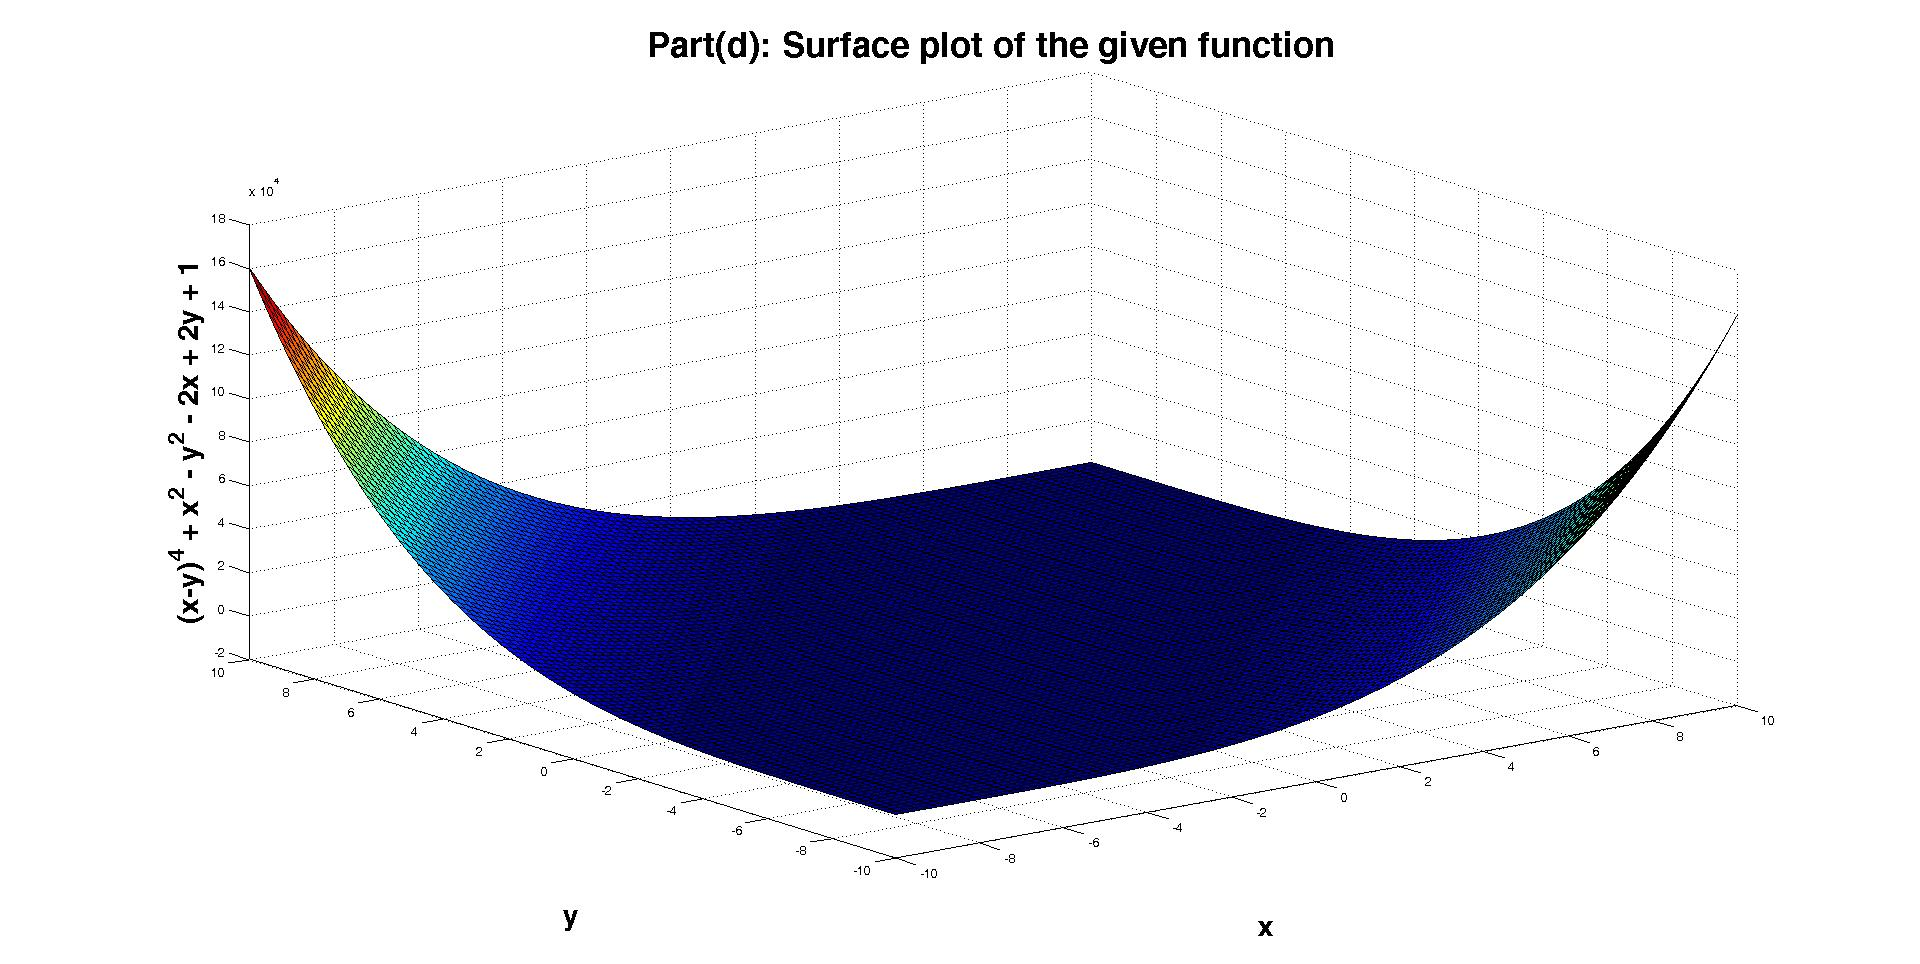
\includegraphics[width=7.in]{plot4} \\
\end{center}\hrule \hrule \hrule 
\end{document}